\documentclass[a4paper]{article}
\usepackage[utf8]{inputenc}
\usepackage{natbib}
\usepackage{graphicx}
\usepackage{xcolor}
\usepackage{booktabs}
\usepackage[ngerman]{babel}
\usepackage[a4paper,left=3cm,right=3cm,bottom=3cm]{geometry}
\usepackage{color}
\usepackage[colorlinks,allcolors=blue]{hyperref}

\let\oldv\verbatim
\let\oldendv\endverbatim

\def\verbatim{\par\setbox0\vbox\bgroup\oldv}
\def\endverbatim{\oldendv\egroup\fboxsep0pt \noindent\colorbox[gray]{0.9}{\usebox0}\par}



\begin{document}

\begin{titlepage}
\title{

\includegraphics{figures/Logo.jpg} \\
\vspace*{1in}
\textbf{PubQuiz-Master}}
\author{Hartmann Ewald\\
        Novosel Florian\\
        Reisinger Lukas\\
		\vspace*{0.5in} \\
		Studiengang Wirtschaftsinformatik\\
        \textbf{FH Campus 02}\\
        Graz, Österreich
       } \date{\today}
%--------------------Make usable space all of page
\setlength{\oddsidemargin}{0in} \setlength{\evensidemargin}{0in}
\setlength{\topmargin}{2in}     \setlength{\headsep}{-.25in}
\setlength{\textwidth}{6.5in}   \setlength{\textheight}{8.5in}
%--------------------Indention
\setlength{\parindent}{1cm}

\maketitle
\thispagestyle{empty}
\setcounter{page}{0}
\end{titlepage}
\clearpage

\begingroup
\hypersetup{linkcolor=black}
\tableofcontents
\endgroup
\clearpage

\section{Allgemeine Beschreibung}
Das Pubquiz - in vielen Grazer Lokalen ein beliebtes Mittel zum Zeitvertreib und Prokrastination für Student:innen. Die Vorbereitung dazu ist oftmals umfangreicher als vermutet. Das Projekt soll hierzu Abhilfe schaffen indem der oder die Benutzer:in auf eine bestehende Datenbank, in der Fragen inklusiver Antwortmöglichkeiten zu verschiedensten Themengebieten vorhanden sind, zugreifen kann. Weiters übernimmt die Anwendung auch die gesamte Validierung der gewählten Antwortmöglichkeit. 

\section{Anforderungsanalyse}

\begin{itemize}
  \item Der oder die Benutzer:in soll den Umfang (Anzahl der Fragen und dessen Schwierigkeit) sowie das jeweilige Themengebiet zu welches sich das Quiz handelt, selbst für jeden Durchlauf bestimmen können. 
  \item Nach jeder Frage soll ein Feedback über die Richtigkeit der gegebenen Antwort dem oder der Benutzer:in geliefert werden.
  \item Zum Abschluss eines Quiz-Durchlaufes soll eine Statistik dem oder der Benutzer:in angezeigt werden.
  \item Der oder die Benutzer:in soll Voreinstellungen für die Quiz hinsichtlich Umfang und Kategorie innerhalb von JSON und XML Dateien hochladen können, beispielsweise um "Favoriten" direkt parat zu haben. Die Validität der Eingabedaten soll überprüft werden, um in weiterer Folge dem oder die Benutzer:in mittels Fehlermeldungen auf ungültige Strukturen oder Dateien hinzuweisen.
\end{itemize}

\section{Systemarchitektur}
Wie in der Abbildung \ref{fig:my_label} ersichtlich, dient die Businesslogik der Anwendung als zentraler Dreh- und Angelpunkt für die jeweiligen Benutzereingaben und darauffolgenden Rückmeldungen. Als Input können entweder vorgefertigte JSON und XML Files dienen, oder auch direkt durch den Benutzer über ein HTML-Formular. Die Validierung von XML Files wird über ein XSD Schema realisiert. Die Aufbereitung zur Anzeige des Eingabe XMLs übernimmt der XSLT Processor. Anfragen werden via Fetch-API an der OpentriviaDB (https://opentdb.com/) gestellt. Die Antwort wird als JSON geparsed und wiederum von der Businesslogik weiterverarbeitet.

\clearpage

\section{Datenmodell}

\begin{figure}[h]
    \centering
    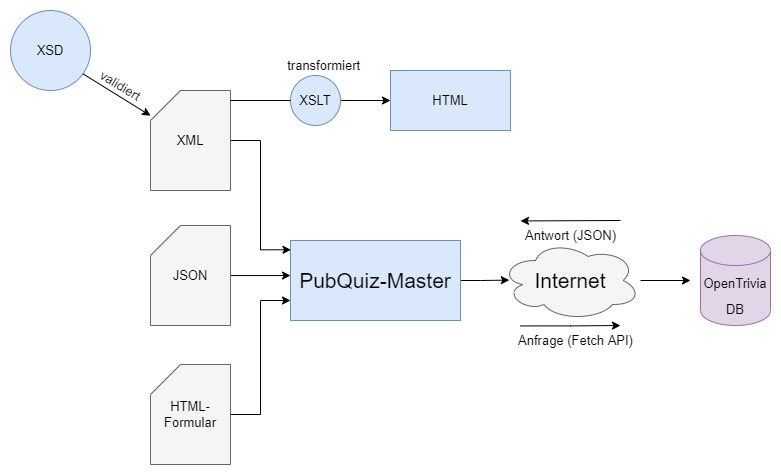
\includegraphics[scale=0.5]{figures/PubQuizMaster4.jpg}
    \caption{Systemarchitektur PubQuiz-Master}
    \label{fig:my_label}
\end{figure}



\textbf{XML:}

\begin{itemize}
  \item \textbf{quizes:} 'quizes' beschreibt den Wurzelknoten. Dieser enthält eine beliebige Anzahl von Elementen des Typs 'Quiz', welches mindestens einmal vorkommen muss.
  \begin{itemize}
  \item \textbf{quiz:} 'quiz' beschreibt einen jeweiligen Quizdurchlauf mit entsprechenden Einstellungen. Das Element beinhaltet die Werte 'amount', 'difficulty' und 'category'. Jedes dieser Elemente muss und darf genau einmal vorkommen.
   \begin{itemize}
  \item \textbf{amount:} Integer Wert der die Anzahl an Fragen im Quiz definiert. Wertebereich 1 - 20. Beispielwert: 8
   \item \textbf{difficulty:} String Wert der die Schwierigkeit im Quiz definiert. Mögliche Werte sind 'easy', 'medium' und 'hard'.
      \item \textbf{category:} Integer Wert der die Kategorie im Quiz definiert. Der Wert beschreibt die jeweilige Kategorie-ID. Wertebereich 9-32. Beispielwert: 11
\end{itemize}
  
\end{itemize}
\end{itemize}
\textbf{Beispiel XML:}
\begin{verbatim}
<quizes>
    <quiz>
        <amount>9</amount>
        <difficulty>easy</difficulty>
        <category>12</category>
    </quiz>
</quizes>
\end{verbatim}
\vspace{0.5cm}
\hspace{-0.51cm}Inhalte des JSON Dokumente beinhalten ein 'Quiz' Objekt, welche ebenfalls die obrigen Attribute inklusiver der im XML definierten erlaubten Wertebereiche.\vspace{0.5cm}

\clearpage
\hspace{-0.5cm}\textbf{Beispiel JSON:}
\begin{verbatim}
{
    "Quiz": {
        "amount": 12,
        "difficulty": "easy",
        "category": 9
    }
}
\end{verbatim}

\section{Schnittstellenbeschreibung}
Als Webservice wurde die von OpenTriviaDB zur Verfügung gestellte API verwendet. Die zugehörige Dokumentation kann \href{https://opentdb.com/api_config.php}{hier} abgerufen werden.

\begin{table}[h]
\centering
\begin{tabular}{@{}lllll@{}}
\toprule
\multicolumn{1}{c}{\textbf{HTTP-Methode}} & \multicolumn{1}{c}{\textbf{Endpoint}} & \multicolumn{1}{c}{\textbf{Beschreibung}}       \\ \midrule
GET                                       & \text{/api\_category.php}             & Einlesen aller verfügbaren Kategorien                      \\
GET                                       & \text{/api.php?amount=}               & Übermittlung der Anzahl an benötigten Fragen \\
GET                                       & \text{/api.php?cat=}                  & Übermittlung der gewünschten Kategorie \\
GET                                       & \text{/api.php?difficulty=}           & Übermittlung der gewünschten Schwierigkeit \\
GET                                       & \text{/api.php?type=multiple}         & Gibt an dass nur Multiple-Choice Fragen gewünscht sind \\ \bottomrule
\end{tabular}
\label{tbl:api}
\end{table}

\section{Projektablauf}

\subsection{Tech Stack}
Die grundlegende Businesslogik wurde in \emph{Javascript} erstellt. Zur generellen Kommunikation mit der OpenTrivia Database wurde eine \emph{Fetch API} verwendet. Das generelle Styling der Webapplikation erfolgte mittels \emph{Tailwind CSS}.

\subsection{Workflow}
Zur gemeinsamen Arbeit am Code und der Versionsverwaltung wurde ein \href{https://gitlab.com/Scrolls8010/mul_projekt_grp_3}{Gitlab Repository} erstellt. Zur einfachen Abstimmung hat die Projektgruppe einen separaten Teams-Kanal angelegt, in dem die gesamte Kommunikation sowie diverse Statusmeetings abgehalten wurden. Die Abstimmung hierzu war sehr einfach und professionell da in dieser Gruppe bereits mehrfach Projekte umgesetzt wurden. Zu Beginn wurden mehrere Themen für mögliche Anwendungen gemeinsam gesucht und evaluiert. Im Anschluss erfolgte eine grobe Aufteilung der Arbeitspakete. Nachdem ein jeweils umfangreicherer Teil fertiggestellt wurde, gab es ein Synch-Meeting zwischen allen Projektmitgliedern.

\subsection{Tasks}
Ewald Hartmann übernahm den Hauptteil der Businesslogik und der Funktionalität rund um die API. FLorian Novosel war Hauptverantwortlicher für die Implementierung der Logik zur Verwendung von XML Dateien als Input sowie dessen Validierung mittels XSL sowie anschließender Transformation in ein HTML Dokument via XSL. Lukas Reisinger war Hauptverantwortlicher für die Erstellung der Projektdokumentation und Informationsbeschaffung zu LateX. Bei etwaigen aufkommenden Fragen von einzelnen Personen wurden diese jeweils kurzfristig innerhalb des Teams gemeinsam geklärt, bzw. bei Unklarheiten zum Projektumfang, mit dem Lektor der Lehrveranstaltung aufgelöst.

\end{document}
